\documentclass[letterpaper,12pt]{report}
\usepackage[english]{babel}							%For internationalization
\usepackage[utf8]{inputenc}							%For character encoding
\usepackage{amsmath}								%For mathematical typesetting
\usepackage{amssymb}								%For mathematical typesetting
\usepackage{graphicx}								%For handling graphics
\usepackage[top=1in, bottom=1in, left=1.5in, right=1in]{geometry}	%Sets required thesis margins
\usepackage[nodisplayskipstretch,doublespacing]{setspace} 		%Sets required thesis double spacing
\usepackage{titlesec} 								%Used to easily redefine section title styles

\newcommand{\be}{\begin{equation}}
\newcommand{\ben}[1]{\begin{equation}\label{#1}}
\newcommand{\ee}{\end{equation}}
\newcommand{\aomega}{\overset{\sim}{\omega}}				%Approximate omega

\title{Vortex Dominated Flows: A High-Order, Conservative Eulerian Simulation Method}
\author{Josh Bevan}
\date{\today}

%Set section formats so chapters, sections, and subsections are 14ish pt
\titleformat{\section}{\large\bfseries}{\thesection}{1em}{}
\titleformat{\subsection}{\normalsize\bfseries}{\thesection}{1em}{}
\titleformat{\chapter}{\large\bfseries}{\thechapter}{1em}{}
	\titlespacing*{\chapter}{0pt}{.7in}{0pt} %Add whitespace above chapter title to get a 2in margin

%Frontmatter----------------------------------------------------------------------
\begin{document}
\pagenumbering{roman} %Roman numbering for frontmatter
\maketitle
\begin{abstract}
\setcounter{page}{2} %Manual page numbering because 'abstract' is annoying
\thispagestyle{plain} %Needed to show page number as pagestyle was reset to 'empty' when \maketitle is called internally
A high-order, conservative Eulerian method is presented for the simulation of vortex dominated inviscid fluid flows. The primitive variable Navier-Stokes equations are recast in the velocity-vorticity form to explicitly enforce conservation of vorticity. The advection of the vorticity is then calculated via a two-step process each time-step: the velocity field is determined by evaluation of the Biot-Savart integral, and then a line-based discontinuous Galerkin (DG) Eulerian spatial discretization scheme is applied. The accuracy and convergence of this method is examined for test cases where an analytical solution exists, as well as more challenging test cases which lack an analytical solution. Of particular interest is the influence the discretization of the calculated velocity field has on the performance of the method.
\end{abstract}

\setcounter{page}{3} %Manual page numbering because 'abstract' is annoying
\chapter*{Acknowledgments}
\begin{singlespace} %Tables should be single spaced
\tableofcontents
\listoftables
\addcontentsline{toc}{section}{List of Tables}
\listoffigures
\addcontentsline{toc}{section}{List of Figures}
\end{singlespace}

%Here we change the pagestyle so that the page number appears top right. We need to redefine the \chapter command to change the default pagestyle from 'plain' to 'myheadings'
\pagestyle{myheadings}
\makeatletter
\renewcommand\chapter{\if@openright\cleardoublepage\else\clearpage\fi
                    \thispagestyle{myheadings}% original style: plain
                    \global\@topnum\z@
                    \@afterindentfalse
                    \secdef\@chapter\@schapter}
\makeatother

%Mainmatter-----------------------------------------------------------------------
\chapter{Introduction}
\pagenumbering{arabic} %Reset to arabic numbering for mainmatter
\section{Problem Formulation}
-DNS expensive \\
-For inviscid vortex dominated flows $\rightarrow$ reformulate from primitive variables to velocity-vorticity \\
-Existing methods: Lagrangian vortex particle methods [Carley, Strain, Leonard] and VTM [Brown]\\
-Difficulty extending to high order: Particle methods (re-meshing), VTM (extended stencil)\\
-Available high order methods unsuitable: FD/FV (extended stencil and smearing), FE (non-conservative, ill-suited for hyperbolic), Spectral (Globally defined vs concentrated sparse vorticity)
\section{Chosen Methods}
-DG: conservative, local, flux funs handle hyperbolicity\\
-Line DG easy implementation for hexahedral meshes. Tensor product points allow possibility of easy biasing along principal flow directions. Allow easy translation of 1D methods for multidimensional domains\\
-Direct evaluation of BS integral: allows investigation of local order refinement effects on global convergence
\section{Thesis Structure}
-Theory: Develop method specific mathematics (DG, VTM, BS, etc)\\
-Methodology: Cover relevant notable implementation specifics (e.g. Solver structure, non-trivial algorithms), present convergence test structure (analytical cases, elliptical blob, 2-D "ring",several interacting patches) vs (convergence rate of: constant order velocity field, linear far field velocity [far= 1 element or X element separation], variable far field velocity order [heuristic?])\\
-Results: Results of matrix of tests (summary with aggregate plots, and selected results)\\
-Discussion: Analytical validation, comparison of velocity field fidelity test, comments on effects of global convergence

%------------------------------------
\chapter{Theory}
\section{Navier-Stokes: Velocity-vorticity form}
If the quantity \textit{vorticity} is defined as
\be \omega = \nabla \times u \ee
Then the traditional form of the Navier-Stokes equations can be recast, assuming an inviscid incompressible flow
\ben{VV3D} \frac{\partial \omega}{\partial t} + u \cdot \nabla \omega - \omega \cdot \nabla u = S(x,t)\ee

There are several benefits to the recast form: explicitly conserving vorticity, sparseness, pressure term need not be solved for... [elaborate]

Restricting  to examining 2-D distributions of vorticity, several simplifications can be made. The originally vectorial vorticity becomes a scalar quantity, all vorticity is directed normal to the plane. As a result, the vortex stretching term in \eqref{VV3D} becomes zero. The only non-zero component of $\omega$ is in the z-direction, however the gradient of the velocity field is zero in the z-direction, so the product is therefore zero. The result is
\ben{VV2D} \frac{\partial \omega}{\partial t} + u \cdot \nabla \omega = S(x,t)\ee
or if instead the second term is expressed in terms of the flux of the vorticity (where $f_i(\omega)=u_i\,\omega$):
\ben{VV2D} \frac{\partial \omega}{\partial t} + \frac{\partial f}{\partial x_i}= S(x,t)\ee

\section{Velocity Field Evaluation: The Biot-Savart Integral}
We shall decide that $\omega$ is the quantity of interest in the solution method. However, if this is the case then the question must be posed: how does one determine the velocity field? For an incompressible flow
\be \nabla^2 u = -\nabla \times \omega \ee
If inverted, the Biot-Savart integral is obtained
\ben{BS} u(x^*) = \int_\Omega K(x^*,x) \times \omega(x) dx \ee
with the singular Biot-Savart kernel
\ben{BSkern} K(x^*,x) = \frac{-1}{4 \pi} \frac{x^*-x}{|x^*-x|^3} \ee

There are several important points to note that are a consequence of this inversion. First, rather than solving the Poisson equation for the entirety of the domain we choose to evaluate the velocity at some subset. For the purposes of advecting the velocity we will only need velocities near the vorticity itself. However, if the number of required velocity evaluation points is roughly proportional to the $N$ DOFs of our vorticity approximation, then it might be expected for the velocity calculations to scale as $\mathcal{O}(N^2)$.

There are numerous methods to reduce the computational complexity of similar N-body type problems to $\mathcal{O}(NlogN)$ or $\mathcal{O}(N)$. Cyclic reduction [Schumann, Sweet 1976], tree-codes [Lindsay/Krasny][Barnes-Hut], and FMM [Greengard] are all possibilities. However, because the velocity field calculation method is essentially decoupled from the discretization of the PDE, there is no a priori assurance that the velocity calculated is of sufficient fidelity to ensure convergence of the overall method (let alone convergence at the order one might expect based on solely the discretization). For maximum flexibility in investigating this dependency of overall convergence on the calculated velocity field we shall eschew more efficient techniques so that we can directly control the fidelity of the velocity field.

The second point to consider regarding the Biot-Savart integral is the singular nature of the exact kernel. Lagrangian point vortex methods have the benefit that the singularity and it's associated non-physical velocities occur in a relatively small region; they assume that the advective effect of the point vortex on itself is negligble [hazy on this, clarify some]. Additionally they will frequently de-singularize the kernel by introducing a core function. The classical one used is the Rosenhead-Moore kernel [ref here]:
\ben{RMkern} K(x^*,x) = \frac{-1}{4 \pi} \frac{x^*-x}{(|x^*-x|^2+\sigma^2)^{3/2}} \ee

The high-order Eulerian approach taken here however means that the Biot-Savart integral diverges everywhere within any of the extended vorticity patches thanks to self-influence.


Expense of calculation (\% of total program?), Self-terms: Subsplitting vs GL quadrature skip vs kernels

\section{Discontinuous Galerkin}
In order to solve \eqref{VV2D} we adopt a method-of-lines approach. We will first spatially discretize the system to obtain the semi-discrete system, then we use an explicit time discretization method to march forward in time. Note that \eqref{VV2D} has the form of a scalar conservation law, with $\omega$ being the conserved quantity. The velocity field that advects the conserved quantity has been calculated by evaluation of the Biot-Savart integral for the current timestep.

Our spatial discretization is at best an approximate solution to \eqref{VV2D}, that we shall denote as $\aomega(x,t)$. Some residual will remain for the approximate solution of the PDE at any time $t$
\ben{VV2D} \frac{\partial \aomega}{\partial t} + \frac{\partial f}{\partial x_i} = R(x)\ee
where we have shown a 1-D case and omitted vorticity sources for simplicity.

The Discontinuous Galerkin (DG) approach attempts to approximately satisfy the PDE in the following way: Seek the best approximation in a finite vector test space $\mathbb{W}_h$  in the $L^2$ norm sense. Minimize the $L^2$ norm by an orthogonal projection of the residual onto $\mathbb{W}_h$. Form a complete basis for $\mathbb{W}_h$ with a set of test functions $\phi_j \in \mathbb{W}_h$, such that the orthogonal projection satisfies:
\be \int_\Omega R(x) \phi_j \;dx = 0 \quad\mbox{for all}\; j\ee
Substituting the residual for our conservation PDE yields:
\be \int_\Omega \frac{\partial \aomega}{\partial t} \, \phi_j \;dx + \int_\Omega \frac{\partial f(\aomega)}{\partial x} \, \phi_j \;dx = 0 \quad\mbox{for all}\; j\ee

Choose the space of piecewise polynomials for the finite dimensional approximation space, and decompose the global domain into K elements where the local approximation space $\overset{k}{\mathbb{V}}_h$ has basis functions $\overset{k}{\psi}_i(x)$ over the local domain $x \in [x_L, x_R]$ (henceforth we drop the element index $k$ for brevity, except when describing two distinct elements that must be distinguished). Note that continuity of vorticity is not enforced across elements, and that the local approximation spaces for each element are independently defined. Finally, take the Bubnov-Galerkin choice of setting the test space to be the same as the approximation space so that $\phi_j=\psi_i \in \mathbb{V}_h$ if $i=j$. The local Mth order approximation to vorticity takes the form

\be \omega(x,t) \approx \aomega(x,t) = \sum_{i=0}^M a_i(t)\psi_i(x)\ee

where $a_i$ is some set of coefficients that are to be determined. The elemental approximating PDE is then

\be \sum_{i=0}^M \left[ \frac{d a_i(t)}{dt}\int_{x_L}^{x_R}\psi_i(x)  \, \phi_j(x) \;dx \right]
+ \int_{x_L}^{x_R} \frac{\partial f(\aomega)}{\partial x} \, \phi_j \;dx = 0 \ee

To reduce the smoothness requirements on the flux, integrate the second term by parts to yield
\ben{DGtemp} \sum_{i=0}^M \left[ \frac{d a_i(t)}{dt}\int_{x_L}^{x_R}\psi_i(x)  \, \phi_j(x) \;dx \right]
+ f\phi_j(x) \Big|^{x_R}_{x_L} 
- \int_{x_L}^{x_R} f(\aomega) \, \frac{d \phi_j(x)}{d x} \;dx = 0 \ee

The local solution offers no way of recovering the global solution, until one realizes that the flux at the element boundaries is multiply defined between elements. The global solution is allowed to be piecewise discontinuous across boundaries, so there is no guarantee that the flux between neighboring elements would agree. To resolve this (and at the same time recover a global solution) define a numerical flux analogous to a Finite Volume Method (FVM) that takes as input the vorticity at the adjacent element boundaries. We will use an upwind flux, where defining the average as $\{\!\{\omega^+\}\!\} = \frac{\omega^++\omega^-}{2}$ and the jump as $[[\omega]]=\omega^+-\omega^-$, yields
\be \hat{f}_{upwind}(x^+,x^-)=u\{\!\{\aomega\}\!\} + \frac{|u|}{2}[[\aomega]]\ee

We would also like to map any element to a computational element by means of a mapping $x=g(X)$ and it's inverse $X=G(x)$. If we set the domain of our computational element to be $X \in [-1, 1]$ and the element size to be $\Delta x = x_R - x_L$, then the mapping is
\be x=g(X)=\frac{X+1}{2}\Delta x + x_L\quad ,\quad X=G(x)=\frac{2(x-x_L)}{\Delta x}+1 \ee

Applying a change of variables using the mapping to \eqref{DGtemp}, accounting for the numerical flux, and being sure to include the determinant of the Jacobian matrix that results from the mapping ($J=g'(X)=\Delta x/2$) in the first integral:
\ben{DGtemp} \frac{\Delta x}{2}	\sum_{i=0}^M \left[ \frac{d a_i}{dt}	\int_{-1}^{1}\psi_i  \, \phi_j \;dX \right]
+\hat{f}\phi_j \Big|^{x_R}_{x_L} 
- \int_{-1}^{1} f(\aomega) \, \frac{d \phi_j}{dX} \;dX = 0 \ee
(Note: no determinant of the Jacobian matrix appears in the second integral because one of the basis functions has been differentiated. When the chain rule is applied during the change of variables an extra $1/g'(X)$ appears that cancels out with the $g'(X)$ that occurred from the change of variables on the integral)

We have purposely left the flux in the second integral unevaluated in terms of the basis functions, as well as the choice of basis functions left as undecided. We defer these choices to a more in depth investigation in Methodology. We also have developed the equations past the initial PDE in a 1-D form. We will shortly show that the basis coefficients are chosen to be nodal values. The 2-D solution will be recovered following the Line-DG methodology [Line-DG Persson citation] element will be composed of a tensor product of two 1-D discretization 

%------------------------------------
\chapter{Methodology}
\section{Overall Solver Structure}
IC and BC initialization, Lagrange pre-calculation, mass and stiffness matrices generation, 2 step spatial discretization, time discretization, post processing
\section{Algorithms of Note}
Vectorized Lagrange evaluation, Lagrange derivatives, etc
\section{Validation and Convergence of Proposed Methods}
(analytical cases, elliptical blob, 2-D "ring",several interacting patches) vs (convergence rate of: constant order velocity field, linear far field velocity [far= 1 element or X element separation], variable far field velocity order [heuristic?])
%------------------------------------
\chapter{Results}
\section{Analytical Test Cases}
\section{Elliptical Blob}
\section{Arbitrary Patch}
\section{Dipole(misuse of term?)}
\section{Vortical System}
%------------------------------------
\chapter{Discussion}
\section{Analytical Validation of Model}
Comparison of existing analytical solutions vs model (Euler vortex, 5th order poly, other Saffmann test cases)
\section{}
%------------------------------------
\chapter{Conclusion}
\section{Weak Formulation}
%------------------------------------
\chapter{Recommendations}
%------------------------------------
\chapter{Literature Cited}
\begin{figure}
\centering
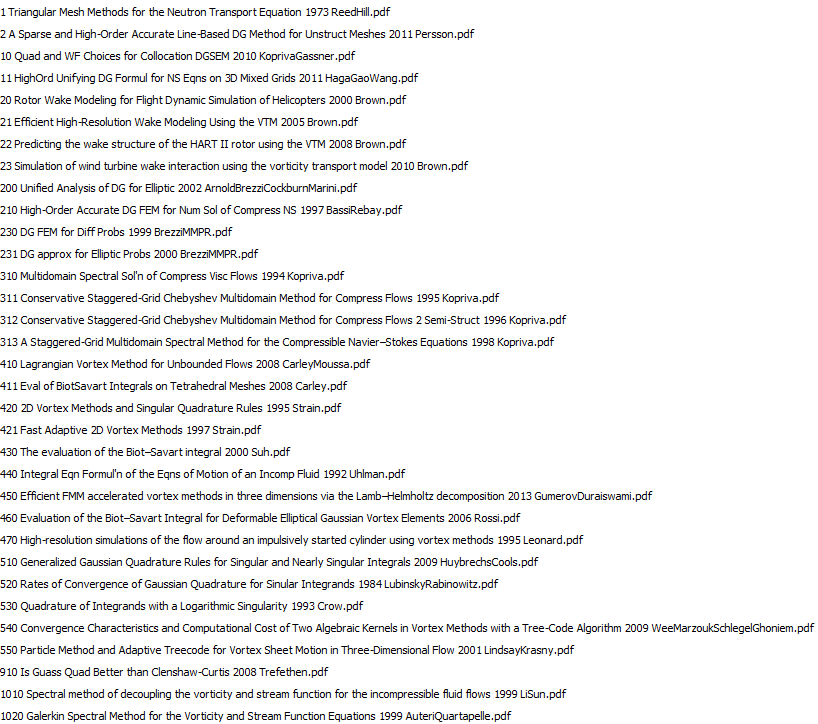
\includegraphics[width=1.4\textwidth]{LitStart.PNG}
\caption{\label{fig:ring}Dirty preliminary lit cited.}
\end{figure}

\end{document}